%%%%%%%%%%%%%%%%%%%%%%%%%%%%%%%%%%%%%%%%%%%%%%%%%%%%%%%%%%%%%%%%
% %
% Due Date %
% Andrew Gibson %
% ECE 351 lab, Section 53 %
% Lab 2 %
% Due 7 Jan 2023 %
% User-Defined Functions %
%https://github.com/gibs0630/ECE351\_Code %
%https://github.com/gibs0630/ECE351\_Reports %
% %
%%%%%%%%%%%%%%%%%%%%%%%%%%%%%%%%%%%%%%%%%%%%%%%%%%%%%%%%%%%%%%%%

\documentclass[12pt,a4paper]{article}
\usepackage[utf8]{inputenc}
\usepackage[greek,english]{babel}
\usepackage{alphabeta} 
\usepackage[pdftex]{graphicx}
\usepackage[top=1in, bottom=1in, left=1in, right=1in]{geometry}
\linespread{1.06}
\setlength{\parskip}{8pt plus2pt minus2pt}
\widowpenalty 10000
\clubpenalty 10000
\newcommand{\eat}[1]{}
\newcommand{\HRule}{\rule{\linewidth}{0.5mm}}
\usepackage[official]{eurosym}
\usepackage{enumitem}
\setlist{nolistsep,noitemsep}
\usepackage[hidelinks]{hyperref}
\usepackage{cite}
\usepackage{lipsum}


\newcommand{\Q}{\bigskip\bfseries Q: }
\newcommand{\A}{\par\textbf{A:} \normalfont}

\hypersetup{colorlinks=true, linkcolor=black, urlcolor=blue}

\begin{document}
%===========================================================
\begin{titlepage}
\begin{center}
% Top 
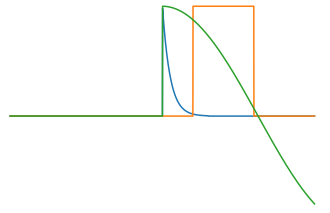
\includegraphics[width=0.55\textwidth]{titlepage_image.png}~\\[2cm]
% Title
\HRule \\[0.4cm]
{ \LARGE 
  \textbf{Project Report for ECE 351}\\[0.4cm]
  \emph{Lab 4: System Step Response Using Convolution}\\[0.4cm]
}
\HRule \\[1.5cm]
% Author
{ \large
  Andrew Gibson \\[0.1cm]
  7 February 2023\\[0.1cm]
  \url{https://github.com/gibs0630/ECE351\_Code}\\[0.1cm]
  \url{https://github.com/gibs0630/ECE351\_Reports}\\[0.1cm]
  %#\texttt{user@cut.ac.cy}
}
\vfill
%\textsc{\Large Cyprus University of Technology}\\[0.4cm]\textsc{\large Department of Electrical Engineering,\\Computer Engineering \& Informatics}\\[0.4cm]
% Bottom
{\large }
 
\end{center}
\end{titlepage}
%\begin{abstract}
%\lipsum[1-2]
%\addtocontents{toc}{\protect\thispagestyle{empty}}
%\end{abstract}
\newpage
%===========================================================
\tableofcontents
\addtocontents{toc}{\protect\thispagestyle{empty}}
\newpage
\setcounter{page}{1}
%===========================================================
%===========================================================
\section{Introduction}\label{sec:intro}
There is a special case what computing convolutions.  If one of them is the unit step function, then the answer will be the integral of the other.

\section{Equations}\label{sec:lit-rev}
Formula's used
unit step function
\[
u(x) = \left\{
        \begin{array}{ll}
            0 & \quad t < 0 \\
            1 & \quad t \geq 0
        \end{array}
    \right.
\]
ramp function
\[
r(x) = \left\{
        \begin{array}{ll}
            0 & \quad t < 0 \\
            t & \quad t \geq 0
        \end{array}
    \right.
\]
discrete convolution with uniform time interval at 1
\[h(t) = \sum_{k=-\infty}^{\infty} {\left [ \sum_{n=0}^{k} {\left [ f_n*g_{k-n}* \Delta t\right ]} \right ]}\]

discrete convolution with uniform time intervals
\[h(t) = \sum_{k=-\infty}^{\infty} {\left [ \sum_{n=0}^{k} {\left [ f_n*g_{k-n}\right ]} \right ]}\]

functions from lab
\[h_1(t) = e^{-2t}(u(t)-u(t-3))\]
\[h_2(t) = u(t-2)-u(t-6)\]
\[h_3(t) = cos(\omega_0 t)u(t)\]


\section{Methodology}\label{sec:meth}
This lab had us create some functions and plot them, discrete convolve them with the unit step function, and then compare those with the mathamatical answer.

\section{Results}\label{sec:res}
\subsection*{Part 1}

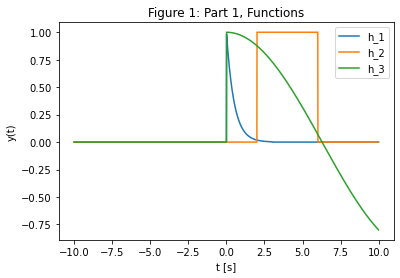
\includegraphics[width=0.55\textwidth]{Figure1.png}\\
The purpose producing Figure 1 was to show the functions as they are.

\subsection*{Part 2}
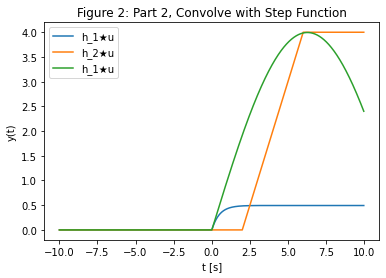
\includegraphics[width=0.55\textwidth]{Figure2.png}\\
Figure 2 shows the functions convolved with the unit step function.\\

The math for the convolution are as follows:
for h$_1$
\[h_1(t)\star u(t) = \int_{-\infty}^\infty \left [ \left (e^{-2\tau}(u(\tau)-u(\tau-3))\right ) \left (u(t-\tau)\right ) d \tau \right ]\]

\[ = \int_{-\infty}^\infty \left [ \left (e^{-2\tau}u(\tau)-e^{-2\tau}u(\tau-3))\right ) \left (u(t-\tau)\right ) d \tau \right ]\]

\[ = \int_{-\infty}^\infty \left [ e^{-2\tau}u(\tau)u(t-\tau) d \tau \right ]- \int_{-\infty}^\infty \left [ e^{-2\tau}u(\tau-3) u(t-\tau) d \tau \right ]\]

\[ = \int_{0}^t \left [ e^{-2\tau}d \tau \right ]u(t)- \int_{-\infty}^\infty \left [ e^{-2\tau}u(\tau-3) u(t-\tau) d \tau \right ]\]

\[ =\left [\frac{1}{-2}e^{-2t} -\frac{1}{-2} \right ]u(t)- \int_{-\infty}^\infty \left [ e^{-2\tau}u(\tau-3) u(t-\tau) d \tau \right ]\]

\[ =\left [\frac{1}{-2}e^{-2t} -\frac{1}{-2} \right ]u(t)- \int_{-\infty}^\infty \left [ e^{-2(\tau-3+3)}u(\tau-3) u(t-\tau) d \tau \right ]\]

\[ =\left [\frac{1}{-2}e^{-2t} -\frac{1}{-2} \right ]u(t)- \int_{-\infty}^\infty \left [ e^{-2(\tau-3)}e^{-6}u(\tau-3) u(t-\tau) d \tau \right ]\]

\[ =\left [\frac{1}{-2}e^{-2t} -\frac{1}{-2} \right ]u(t)- e^{-6}\int_{-\infty}^\infty \left [ e^{-2(\tau-3)}u(\tau-3) u(t-\tau) d \tau \right ]\]

\[ =\left [\frac{1}{-2}e^{-2t} -\frac{1}{-2} \right ]u(t)- e^{-6} \left [ \left( e^{-2(t-3)}u(t-3)\right )\star u(t) \right ]\]

\[ =\left [\frac{1}{-2}e^{-2t} -\frac{1}{-2} \right ]u(t)- e^{-6} \left [ \left( e^{-2(t)}u(t)\right )\star u(t) \right ]_{t-3} \]

\[ =\left [\frac{1}{-2}e^{-2t} -\frac{1}{-2} \right ]u(t)- e^{-6} \left [\left [\frac{1}{-2}e^{-2t} -\frac{1}{-2} \right ]u(t)\right ]_{t-3} \]

\[ =\left [\frac{1}{-2}e^{-2t} -\frac{1}{-2} \right ]u(t)- e^{-6} \left [\left [\frac{1}{-2}e^{-2(t-3)} -\frac{1}{-2} \right ]u(t-3)\right ] \]

\[ =\left [\frac{1}{-2}e^{-2t} -\frac{1}{-2} \right ]u(t)- \left[  \frac{e^{-6}}{-2}e^{-2(t-3)} -\frac{1}{-2}e^{-6} \right ]u(t-3) \]

\[ =\left [\frac{1}{-2}e^{-2t} -\frac{1}{-2} \right ]u(t)-  \left [\frac{1}{-2}e^{-2(t-3)-6} -\frac{1}{-2}e^{-6} \right ]u(t-3) \]

\[ =\left [\frac{1}{-2}e^{-2t} -\frac{1}{-2} \right ]u(t)-  \left[\frac{1}{-2}e^{-2t} -\frac{1}{-2}e^{-6} \right ]u(t-3)\]

\[ =\frac{1}{2}\left(\left [1-e^{-2t} \right ]u(t)-  \left[e^{-6}-e^{-2t}  \right ]u(t-3) \right)\]

for h$_2$
\[h_2(t) \star u(t-2) = \left (u(t-2)-u(t-6)\right )\star u(t-2)\]

\[ = \left (u(t-2)\star u(t)\right )- \left (u(t-6)\star u(t)\right )\]

\[ = \left [u(t)\star u(t)\right ]_{t-2}- \left [u(t)\star u(t)\right ]_{t-6}\]

\[ = \left [\int_{-\infty}^\infty \left [ \left (u(\tau)\right ) \left (u(t-\tau)\right ) d \tau \right ] \right ]_{t-2}- \left [u(t)\star u(t)\right ]_{t-6}\]

\[ = \left [\int_{0}^t \left [ d \tau \right ] u(t)\right ]_{t-2}- \left [u(t)\star u(t)\right ]_{t-6}\]

\[ = \left [ \left [(t)-(0) \right ] u(t)\right ]_{t-2}- \left [u(t)\star u(t)\right ]_{t-6}\]

\[ = (t-2) u(t-2)- \left [u(t)\star u(t)\right ]_{t-6}\]

\[ = (t-2)u(t-2)-(t-6)u(t-6)\]

for h$_3$
\[h_3(t) \star u(t) =\int_{-\infty}^\infty \left [ \left (cos(\omega_0 \tau)u(\tau)\right ) \left (u(t-\tau)\right ) d \tau \right ]\]

\[ =\int_{0}^t \left [ cos(\omega_0 \tau) d \tau \right ]u(t)\]

\[ =\left [ \frac{1}{\omega_0} sin(\omega_0 (t))-\frac{1}{\omega_0} sin(\omega_0 (0)) \right ]u(t)\]

\[ = \frac{1}{\omega_0} sin(\omega_0 (t))u(t)\]

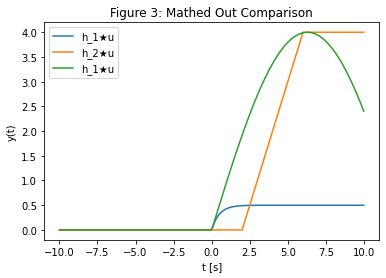
\includegraphics[width=0.55\textwidth]{Figure3.png}\\
Figure 3 shows the functions that were generated after the math was done, and they match up very closely.  These functions just so happen to be integrals of the original functions, as attributed to the special case where a function convolved with the unit step function is the integral of said function.\\


\section{Questions}\label{sec:res}

\Q 1. Leave any feedback on the clarity of lab tasks, expectations, and deliverables.
\A 1. Because my convolution assumed that the index started at zero, I had to rewrite my function entirely in order to accommodate that. while I was fixing that I also corrected for the change in amplitude based on the step size.


%\lipsum[7-8]\cite{knuthwebsite}
%===========================================================
%===========================================================
\bibliographystyle{ieeetr}
\bibliography{refs}
\end{document} 
Annotations











